\documentclass[10pt]{article}

\usepackage[utf8]{inputenc}
\usepackage{floatrow}

\usepackage{algorithm}
\usepackage{algorithmic}
\usepackage[T1]{fontenc}
\usepackage{enumitem}
\usepackage{hyperref}
\usepackage{graphicx}
\usepackage{color}
\usepackage{listings}
\usepackage{wrapfig}
\usepackage{amsfonts}
\usepackage{amsmath}
\usepackage{mathtools}
\usepackage[hmargin=1.25in,vmargin=1.25in]{geometry}

%title setup
\title{Projet informatique: Honshu (Lot A)}
\author{
			Romain PEREIRA\\
			Douha OURIMI\\
			Afizullah RAHMANY\\
			Guangyue CHEN
}
\date{02/03/2018}

% table of contents setup
\renewcommand{\contentsname}{Sommaire}
\usepackage{etoolbox}
\patchcmd{\thebibliography}{\section*{\refname}}{}{}{}

\hypersetup{
    colorlinks,
    citecolor=black,
    filecolor=black,
    linkcolor=blue,
    urlcolor=red
}
			
\begin{document}
	\maketitle
	\tableofcontents
	\newpage
	\section*{Préambule}
		Ce projet est réalisé dans le cadre de nos études à l'ENSIIE.
		L'objectif est de prendre en main des outils de 'programmation agile',
		en developpant un jeu de carte: le Honshu.
	\newline
	\begin{figure}[H]
		\begin{center}
			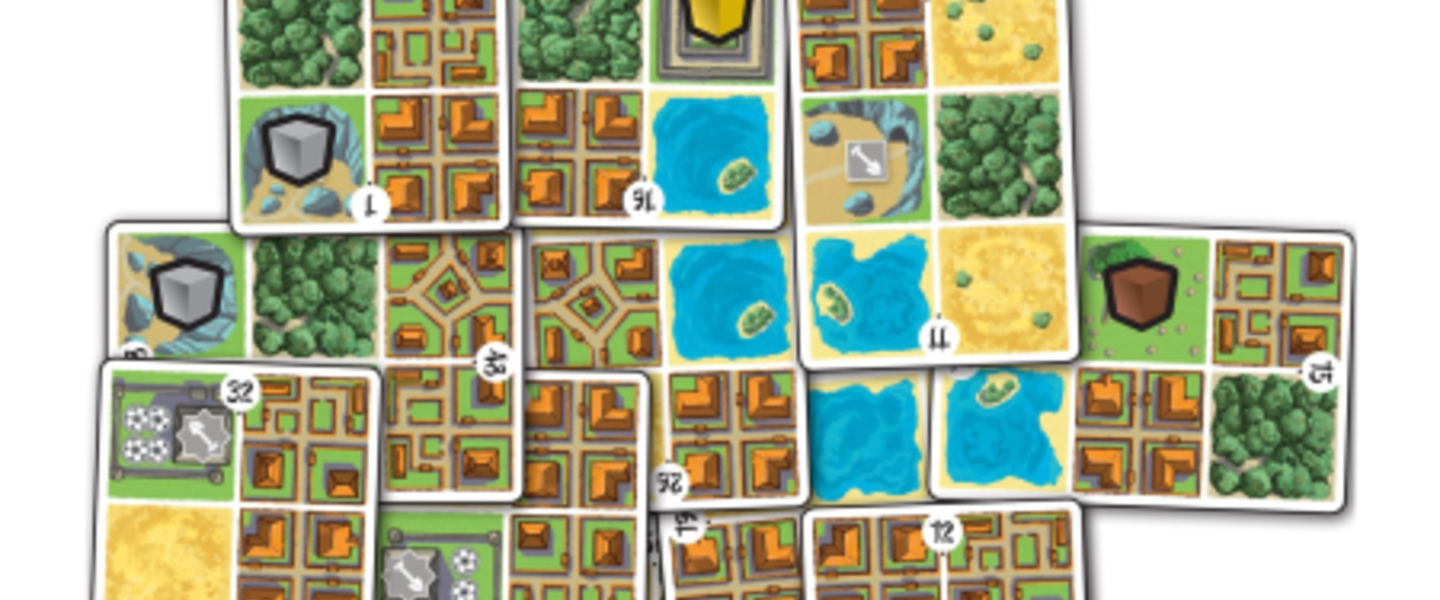
\includegraphics[height=6cm,keepaspectratio]{../images/honshu.png}
		\end{center}
		\caption{\textit{Plateau de jeu}}
		\label{honshu_introduction}
	\end{figure}

	\section{Introduction}
		Ce document rapporte le travail effectué entre le 2 Mars 2018, et le 25 Mars 2018.
		Cette 1ère partie semble être la plus importante du projet:
		nous devons prendre en main les différents outils, structurer le projet,
		puis finalement, concevoir les structures de données et la logique global du programme.
		Une mauvaise conception à ce niveau risque de nous pénaliser sur le reste du projet,
		c'est pourquoi tous les choix techniques seront amplement justifiés au
		regard des futurs lots à rendre.
	\newpage
	
	\newpage
	\section{Rapport lot A}
		\subsection{Organisation du projet, les dates clefs}
			\subsubsection{03/03/18 -> 10/03/18 : préparation du dépot}
				\paragraph{03/03/18 : préparation de l'espace de travail.}
				- Creation des comptes et de l'équipe Gitlab/Trello.\newline
				- Création du dépot Git, et organisation du projet:
				\begin{itemize}
					\item "src" : dossier contenant les sources '.c' du projet
					\item "includes" : dossier contenant les sources '.h' du projet
					\item "tests" : dossier contenant les fichiers tests ('.c' et '.h')
					\item "bin" : dossier contenant les binaires (executables et bibliothèques)
					\item "obj" : dossier temporaire contenant les fichiers objets (compilés)
					\item "doc" : dossier contenant la documentation generé via Doxygen
					\item "Makefile" : pour compiler le projet
					\item ".gitignore" : .gitignore généré via "https://www.gitignore.io/" (afin de ne pas envoyer de fichier compiler et de fichier Latex)
					\item "README.md" : un README indiquant les procédures d'installation du projet/règles du Makefile
					\item "rapport" : dossier contenant des prises de notes pour les rapports.
				\end{itemize}
				Toutes les procédures (compilation, génération de la documentation, tests)
				ont été automatisées dans le Makefile afin de gagner du temps lors du développement.

				\paragraph{07/03/18 : Brainstorming.}\label{Brainstorming}
				Nous nous sommes réunis ce Mercredi matin entre 9h et 11h.
				\begin{itemize}
					\item Installation des outils sur les ordinateurs de Douha et Guangyue
					\item Lecture et demystification du sujet ensemble
					\item Apprentissage des règles du jeu. (nottement à l'aide de la vidéo: \cite{video_regle_jeu}
					\item Réflexion autour de l'implémentation.
				\end{itemize}
				
				\paragraph{08/03/18 : automatisation de l'installation des dépendances.}
					Ajout d'un script shell ("configure.sh") s'occupant d'installer les dépendances sous Linux/MacOSX.

				\paragraph{10/03/18 : début de la rédaction du rapport.}
					Début de la rédaction au propre de ce rapport.
					Les rapports seront rédigés sous Latex (un template est fourni dans le dépot: "rapport/template.tex".
					
			\subsubsection{10/03/18 -> 16/03/18 : 1ère implémentation du jeu}
				Le brainstorming (\ref{Brainstorming}) a posé les bases de l'implémentation techniques.\newline
				Pendant cette période, l'idée était donc d'avoir un prototype qui tourne,
				avec des fonctions 'à trous', que chacun remplirait en se séparant le travail.
				
				\textit{Romain} : Cependant, voulant avoir une 1ère version du jeu rapidement, j'ai fait du zèle
				et j'ai programmé presque l'intégralité du jeu seul.

				\textit{Guangyue} : Cependant, j'ai programmé les codes des fichiers dans le dossier : "tests" .
				
				\paragraph{16/03/18 : entretien avec notre encadrant}
					Pendant l'entretien de la séance encadré, il est ressorti que cette méthode de
					fonctionnement n'est pas bonne: la quantité de travail n'est pas bien repartie entre
					les membres du groupe, et tous les membres ne se sentent pas profondément intégrés au projet.
					Il est important que chaque membre soit intégré et investi dans le projet, afin d'être motivé pour le travail en équipe.
					C'est pourquoi, pendant ce week-end, nous reflechissons à une restructuration du projet qui se suivra par une réunion Lundi soir.(\ref{19_03_18})

			\subsubsection{19/03/18 -> 25/03/18 : 2ème implémentation du jeu en équipe}
					\paragraph{19/03/18 : restructuration du projet}\label{19_03_18}
					Après le premier entretien, nous avons alors décidé de nous réunir le lundi 18/03
					afin de faire un point sur l’avancement du projet et l’organisation du travail.
					Nous avons remis en question la présentation du Trello mais au final elle nous a paru efficace .
					En effet cette présentation permet de voir exactement ce qui doit être fait, ce qui est
					en train d’être fait et ce qui est terminé et par qui cela a été fait. 
					Nous sommes alors passé au projet et nous nous sommes de nouveau concertés sur les structures,
					vérifié que tout le monde les a bien comprises et surtout nous avons décidé de commenter en
					français et non en anglais comme au départ. D’une certaine manière tous les fichiers .c et .h on
					du être repris à 0 par chacun de nous.
					
					\textit{Guangyue} : Pendant le réunion, nous discutons l'architecture ensemble .
					Après la Révision de l'architecture du code , j'ai corrigé les codes des "tests" ,
					et j'ai programmé les fonctions dans les fichiers qui sont dans  le dossier : "src" .

					
				\paragraph{25/03/18 : vérification des tests unitaires :}
					dernier jour avant le rendu, on se dépèche d'intégrer le code de tout le monde,
					et que ca compile sans erreurs. On commence à debogger à l'aide de valgrind.
		\newpage
		\subsection{Détails techniques de l'implémentation}
			\subsubsection{Structure de données}
				On représente une \textbf{case} par:
				\begin{itemize}[label=-]
					\item type : ville, lac, plaine ...
					\item une \textbf{case} au dessus sur la grille (pouvant être nulle)
					\item une \textbf{case} en dessous sur la grille (pouvant être nulle)
					\item la \textbf{tuile} a laquelle cette \textbf{case} appartient
				\end{itemize}
				On représente une \textbf{tuile} par:
				\begin{itemize}[label=-]
					\item 6 \textbf{cases}
					\item une rotation
					\item 1 position sur la carte (la \textbf{case} en haut à gauche de la \textbf{tuile} est l'origine)
				\end{itemize}
				On représente une \textbf{grille} par:
				\begin{itemize}[label=-]
					\item un entier 'n'
					\item un tableau $n*n$ de \textbf{cases} (pouvant être nulle)
				\end{itemize}
				On représente une \textbf{partie} par:
				\begin{itemize}[label=-]
					\item une \textbf{grille}
					\item un tableau de \textbf{tuiles}
				\end{itemize}
				
				Ces structures de données nous permettent de représenter une partie de Honshu efficacement en mémoire,
				et facilite l'implémentation des algorithmes. Pour une \textbf{partie}, avec une \textbf{grille} de taille $n$
				et $m$ tuiles, la complexité spatiale est de l'ordre de:
				
				\[ 8n^2 + 6 * 32 * m + o(n^2) + o(m) \]
								
				\begin{itemize}[label=-]
					\item $8n^2$ : espace mémoire de la grille (tableau de $n^2$ pointeurs)
					\item $6 * 32 * m$ : espace mémoire des tuiles, une tuile contenant 6 cases, et 1 case faisant environ 32 octets.
				\end{itemize}

			\newpage
			\subsubsection{Algorithme / complexité temporelle}
			
				Grâce à ces structures de données, nous pouvons, a n'importe quel instant, accéder à une case (et donc à sa tuile associé) en $O(1)$.
				
				\paragraph{Tests d'insertion d'une tuile :}
					permet de savoir si une tuile peut être insérée à une coordonnée donnée sur la grille (en respectant les règles d'insertions)
						\begin{algorithm}
							\caption{Tests d'insertion d'une tuile}
							\begin{algorithmic}
								\REQUIRE une \textit{grille} ; une \textit{tuile} ; $0 \leq x, y < n$
								\ENSURE Renvoie VRAI ou FAUX, si \textit{tuile} peut être ajoutée à \textit{grille} en \textit{(x, y)}
								\STATE \textit{compteur} $\leftarrow$ 0
								\FOR{Chaque \textit{case, (dx, dy)} de \textit{tuile}}
									\STATE \textit{dessous} $\leftarrow$ \textit{grille}.cases(x + \textit{dx}, y + \textit{dy})
									\IF{\textit{dessous} != NULL}
										\STATE \textit{compteur} = \textit{compteur} + 1
										\IF{\textit{dessous}.type == LAC}
											\STATE Renvoyer FAUX (tentative d'insertion sur un lac)
										\ENDIF
									\ENDIF
									\IF {\textit{compteur} == 0}
										\STATE Renvoyer FAUX (aucunes cases en dessous de la tuile a inséré)
									\ENDIF
								\ENDFOR
								\FOR{Chaque 'tuile' \textit{dessous} sous \textit{tuile}}
									\STATE $x \leftarrow$ Compter le nombre de cases recouvertes de \textit{dessous}
									\STATE $y \leftarrow$ Compter le nombre de cases que \textit{tuile} recouvrirait sur \textit{dessous}
									\IF{$x + y == 6$}
										\STATE Renvoyer FAUX (la tuile \textit{dessous} serait entierement recouverte
									\ENDIF
								\ENDFOR
								\STATE Renvoyer VRAI (tous les tests sont passés)
							\end{algorithmic}
						\end{algorithm}
						Cet algorithme a une complexité en $O(1)$.

				\newpage
				\paragraph{Insertion d'une tuile :}
					aucun test d'insertion n'est à proprement effectué ici. Un simple jeu de pointeurs relie les cases entre elles
					afin d'assurer l'intégrité de nos structures de données. Cet algorithme a une complexité en $O(1)$.
					
					\begin{algorithm}
						\caption{Ajout d'une tuile}
						\begin{algorithmic}
							\REQUIRE une \textit{grille} ; une \textit{tuile} ; $0 \leq x, y < n$
							\ENSURE Ajoutes \textit{tuile} à \textit{grille}
							\FOR{Chaque \textit{case, (dx, dy)} de \textit{tuile}}
								\STATE \textit{dessous} $\leftarrow$ \textit{grille}.cases(x + \textit{dx}, y + \textit{dy})
								\STATE \textit{case}.au\_dessus $\leftarrow$ NULL
								\STATE \textit{case}.au\_dessous $\leftarrow$ \textit{dessous}
								\IF{\textit{dessous} != NULL}
									\STATE \textit{dessous}.au\_dessus $\leftarrow$ \textit{case}
								\ENDIF
								\STATE \textit{grille}.cases(x + dx, y + dy) $\leftarrow$ \textit{case}
							\ENDFOR
						\end{algorithmic}
					\end{algorithm}

				\paragraph{Recuperer le village associé à une ville :}
					Cet algorithme se programme sur le modèle d'un parcours en largeur. \cite{parcours_en_largeur}
					Il a une complexité en $O(T)$, où $T$ est la taille du village associé à la case.
					\begin{algorithm}
						\caption{Taille d'un village associé à une case : T(x, y)}
						\begin{algorithmic}
							\REQUIRE une \textit{grille} ; $0 \leq x, y < n$
							\ENSURE $T(x, y)$
							\STATE $T \leftarrow 0$
							\IF{\textit{grille}.cases(x, y).type != VILLE}
								\STATE Renvoyer $T = 0$
							\ENDIF
							\STATE Soit \textit{file}, une file.
							\STATE \textit{file}.ajout(x, y)
							\STATE Marquer \textit{grille}.cases(x, y) comme visité
							\WHILE{\textit{file}.nonVide()}
								\STATE $T = T + 1$
								\STATE $(xi, yi) \leftarrow$ \textit{file}.pop()
								\STATE \textit{case} $\leftarrow$ \textit{grille}.cases(xi, yi)
								\STATE Marquer \textit{case} comme 'visité'
								\FOR{Chaque \textit{voisin} de \textit{case}}
									\IF{\textit{voisin}.type == VILLE \textit{et} \textit{voisin}.nonVisite()}
										\STATE \textit{file}.ajout(\textit{voisin}.x, \textit{voisin}.y)
										\STATE Marquer \textit{voisin} comme visité
									\ENDIF
								\ENDFOR
							\ENDWHILE
							\STATE Renvoyer $T$
						\end{algorithmic}
					\end{algorithm}
				
				\newpage
				\paragraph{Supprimer une tuile de la grille :}
					fonction recursive qui s'applique sur les tuiles au dessus de celle qu'on supprime, afin d'assurer l'intégrité de la grille.
					\begin{algorithm}
						\caption{Supprime une tuile de la grille (et les tuiles qui en dépendent)}
						\begin{algorithmic}
							\REQUIRE une \textit{grille} ; une \textit{tuile} ; $0 \leq x, y < n$
							\ENSURE Supprimes la \textit{tuile} de la \textit{grille}
							\STATE Supprimer les cases de \textit{tuile} de la grille.
							\FOR{Chaque 'tuile' \textit{dessus} au dessus \textit{tuile}}
								\IF{\textit{dessus} ne respecte plus les règles d'insertion}
									\STATE Supprimer \textit{dessus} de la grille (récursivement)
								\ENDIF
							\ENDFOR
							\STATE Renvoyer $T$
						\end{algorithmic}
					\end{algorithm}

					\paragraph{tests tous les autres fonctions qui sont déjà écrits :}
					CUnit est une combinaison d'un framework indépendant de la plate-forme avec diverses interfaces utilisateur. Le framework de base fournit un support de base pour gérer un registre de test, des suites et des cas de test. Les interfaces utilisateur facilitent l'interaction avec le framework pour exécuter des tests et afficher les résultats.
					Tout d'abord, opérez sur chaque structure. Ensuite, testez chaque fonction dans chaque fichier "*.test.c" . Parce que c'est un test en boîte blanche, pour chaque fonction , on conçoit la situation spécifique qu'il accomplissait, et il conçoit tous les résultats possibles et les compare au résultat courant. Finalement, nous avons constaté que tous les tests ont réussi et que toutes les fonctions écrites ont bien marché. 

	\newpage
	
	\section{Références}
		\begin{thebibliography}{}
			\bibitem{video_regle_jeu}
				Vidéorègle jeu de société "Honshu",\newline
				http://videoregles.net/, 6 Sept. 2017,\newline
				\href{https://www.youtube.com/watch?v=WHD6B\_NCd-4}{\textit{https://www.youtube.com/watch?v=WHD6B\_NCd-4}}.

			\bibitem{parcours_en_largeur}
				Algorithme de parcours en largeur,\newline
				Wikipédia, 11 octobre 2017 à 16:40.,\newline
				\href{https://fr.wikipedia.org/wiki/Algorithme\_de\_parcours\_en\_largeur}{\textit{https://fr.wikipedia.org/wiki/Algorithme\_de\_parcours\_en\_largeur}}.
    
		\end{thebibliography}

\end{document}
